%% defense.tex
%% Copyright 2022 Tom M. Ragonneau
%
% This work may be distributed and/or modified under the
% conditions of the LaTeX Project Public License, either version 1.3
% of this license or (at your option) any later version.
% The latest version of this license is in
%   http://www.latex-project.org/lppl.txt
% and version 1.3 or later is part of all distributions of LaTeX
% version 2005/12/01 or later.
%
% This work has the LPPL maintenance status `maintained'.
%
% The Current Maintainer of this work is Tom M. Ragonneau.
\documentclass{polyu-presentation}
\usepackage{microtype}
\usepackage{booktabs}

% List of hyphenation exceptions for US English
% Source: https://ctan.org/tex-archive/info/digests/tugboat/hyphenex
\input{ushyphex}

% Bibliographical resources
\addbibresource{ragonneau-bib/strings.bib}
\addbibresource{ragonneau-bib/optim.bib}

% Dedicated mathematical macros
\usepackage{xargs}
\newcommand{\auglag}{\mathcal{L}_{\mathsf{A}}}
\newcommand{\auglagalt}{\tilde{\mathcal{L}}_{\mathsf{A}}}
\newcommand{\con}[1][]{c\ifthenelse{\equal{#1}{}}{}{_{#1}}}
\newcommandx{\conm}[2][1={},2={}]{\hat{c}\ifthenelse{\equal{#2}{}}{}{_{#2}}\ifthenelse{\equal{#1}{}}{}{^{#1}}}
\newcommand{\fset}{\Omega}
\newcommand{\ieq}{\mathcal{E}}
\newcommand{\iub}{\mathcal{I}}
\newcommand{\iter}[1][]{x\ifthenelse{\equal{#1}{}}{}{^{#1}}}
\newcommand{\lag}[1][]{\mathcal{L}\ifthenelse{\equal{#1}{}}{}{^{#1}}}
\newcommand{\lagalt}[1][]{\widetilde{\mathcal{L}}\ifthenelse{\equal{#1}{}}{}{^{#1}}}
\newcommand{\lagm}[1][]{\hat{\mathcal{L}}\ifthenelse{\equal{#1}{}}{}{^{#1}}}
\newcommand{\lagp}[1][]{L\ifthenelse{\equal{#1}{}}{}{_{#1}}}
\newcommand{\lm}[1][]{\lambda\ifthenelse{\equal{#1}{}}{}{^{#1}}}
\newcommand{\lpoly}{\mathscr{L}(\R^n)}
\newcommand{\merit}[1][]{\varphi\ifthenelse{\equal{#1}{}}{}{^{#1}}}
\newcommand{\meritm}[1][]{\hat{\varphi}\ifthenelse{\equal{#1}{}}{}{^{#1}}}
\newcommand{\nstep}[1][]{n\ifthenelse{\equal{#1}{}}{}{^{#1}}}
\newcommand{\nstepalt}[1][]{\bar{n}\ifthenelse{\equal{#1}{}}{}{^{#1}}}
\newcommand{\obj}{f}
\newcommand{\objm}[1][]{\hat{f}\ifthenelse{\equal{#1}{}}{}{^{#1}}}
\newcommand{\objmalt}[1][]{\tilde{f}\ifthenelse{\equal{#1}{}}{}{^{#1}}}
\newcommand{\pstep}[1][]{p\ifthenelse{\equal{#1}{}}{}{^{#1}}}
\newcommand{\qpoly}{\mathscr{Q}(\R^n)}
\newcommand{\rad}[1][]{\Delta\ifthenelse{\equal{#1}{}}{}{@\!^{#1}}}
\newcommand{\radlb}[1][]{\delta\ifthenelse{\equal{#1}{}}{}{^{#1}}}
\newcommand{\ratio}[1][]{\rho\ifthenelse{\equal{#1}{}}{}{^{#1}}}
\newcommand{\rstep}[1][]{r\ifthenelse{\equal{#1}{}}{}{^{#1}}}
\newcommand{\sstep}[1][]{s\ifthenelse{\equal{#1}{}}{}{^{#1}}}
\newcommand{\step}[1][]{d\ifthenelse{\equal{#1}{}}{}{^{#1}}}
\newcommand{\tstep}[1][]{t\ifthenelse{\equal{#1}{}}{}{^{#1}}}
\newcommand{\xl}{l}
\newcommand{\xpb}[1][]{\mathcal{P}}
\newcommand{\xpt}[1][]{\mathcal{Y}\ifthenelse{\equal{#1}{}}{}{^{#1}}}
\newcommand{\xsv}[1][]{\mathcal{S}}
\newcommand{\xu}{u}

% If-Then-Else function for pgfplots
\pgfmathdeclarefunction{ifthenelsefpu}{3}{\pgfmathparse{#1*#2 + !#1*#3}}

% Performance and data profiles
\usepackage{xstring}
\newcommand{\drawprofiles}[4]{%
    \def\selectsolvers{#2}%
    \def\selectcsv{figures/#3}%
    \def\selectprofile{#4}%
    \ifthenelse{\equal{#1}{performance}}{%
        \def\selectxlabel{$\log_2(\text{perf.\ ratio})$}%
        \def\selectylabel{Perf.\ profiles ($\tau = 10^{-#4}$)}%
    }{%
        \def\selectxlabel{Number of simplex gradients}%
        \def\selectylabel{Data profiles ($\tau = 10^{-#4}$)}%
    }
    \input{figures/profiles.tex}%
}
\newcommand{\drawperformanceprofiles}[3]{\drawprofiles{performance}{#1}{#2}{#3}}
\newcommand{\drawdataprofiles}[3]{\drawprofiles{data}{#1}{#2}{#3}}

\title{Model-Based DFO Methods and Software}
\subtitle{Ph.D. thesis defense}
\author[Tom M. Ragonneau]{\texorpdfstring{
    Tom M. Ragonneau\\
    \footnotesize Co-supervised by Dr.\ Zaikun Zhang and Prof.\ Xiaojun Chen
}{Tom M. Ragonneau}}
\institute[PolyU AMA]{
    Department of Applied Mathematics\\
    The Hong Kong Polytechnic University
}
\date{December 6, 2022}
\titlegraphic{}

\begin{document}

\begin{frame}
    \frametitle{What is DFO?}
    
	Derivative-free optimization (DFO) aims at solving
    \begin{equation*}
        \min_{\iter \in \fset \subseteq \R^n} \obj(x)
    \end{equation*}
    using only \alert{function values}.
    Typically,~$\obj$ is a \alert{blackbox}.

    \medskip

    \begin{center}
        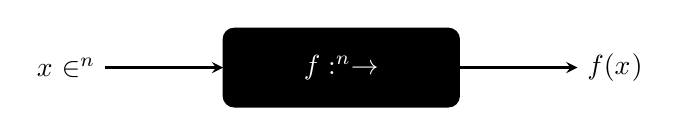
\begin{tikzpicture}
            \draw[rounded corners,fill] (0,0) rectangle (3,1);
            \node[text=white] at (1.5,0.5) {$\obj : \R^n \to \R$};
            \draw[-stealth,thick] (-1.5,0.5) -- (0,0.5);
            \node[left] at (-1.5,0.5) {$\iter \in \R^n$};
            \draw[-stealth,thick] (3,0.5) -- (4.5,0.5);
            \node[right] at (4.5,0.5) {$\obj(\iter)$};
        \end{tikzpicture}
    \end{center}

    \medskip
    
    \begin{block}{}
        \begin{enumerate}
            \item $f$ may be smooth, but derivatives \alert{cannot} be evaluated.
            \item Each function evaluation is \alert{expensive}.
            \item The \alert{computational cost} is the number of function evaluations.
            \item Do \alert{not} use DFO if any kind of first order information is available.
        \end{enumerate}
    \end{block}
\end{frame}

\begin{frame}
    \frametitle{Examples of DFO problems}

    \begin{enumerate}
        \item Academic examples
        \begin{enumerate}
            \item Automatic error analysis \parencite{Higham_1993,Higham_2002}.
            \item Optimization methods tuning \parencite{Audet_Orban_2006}.
            \item \dots
        \end{enumerate}
        \item Engineering and industrial examples
        \begin{enumerate}
            \item \alert<2>{Hyperparameter tuning} \parencite{Ghanbari_Scheinberg_2017}.
            \item Aeroacoustic shape design \parencite{Marsden_2004,Marsden_Etal_2004}.
            \item Computational fluid dynamics \parencite{Duvigneau_Visonneau_2004}.
            \item \alert<2>{Aircraft engineering}~\parencite{Gazaix_Etal_2019}.
            \item Computational nuclear physics \parencite{Eldred_Etal_2022}.
            \item \dots
        \end{enumerate}
    \end{enumerate}

    \medskip

    \pause
    \begin{block}{}
        In what follows, we detail two examples from \alert{machine learning} and \alert{MDO}.
    \end{block}
\end{frame}

\begin{frame}
    \frametitle{Hyperparameter tuning in machine learning}

    \begin{center}
        \begin{tikzpicture}
			\uncover<2>{
				\draw[rounded corners,pattern=north east lines,pattern color=DarkOrchid,fill opacity=0.3] (8,3) rectangle (11,4.5);
			}
			\draw[thick,rounded corners] (0,0) rectangle (3,1.5);
			\draw[thick,rounded corners] (0,4) rectangle (3,5.5);
			\draw[thick,rounded corners] (4,2) rectangle (7,3.5);
			\draw[thick,rounded corners] (8,1) rectangle (11,2.5);
			\draw[thick,rounded corners] (8,3) rectangle (11,4.5);
			\draw[thick,-stealth] (3,1) -- (5.5,1) -- (5.5,2);
			\draw[thick] (3,0.5) -- (7.5,0.5) -- (7.5,2.5) -- (7,2.5);
			\draw[thick,-stealth] (7.5,1.75) -- (8,1.75);
			\draw[thick] (3,4.75) -- (7.5,4.75) -- (7.5,3) -- (7,3);
			\draw[thick,-stealth] (7.5,3.75) -- (8,3.75);
			\node at (0.6,0.75) {\includegraphics[height=0.75cm]{images/ml/presentation.png}};
			\node at (0.6,4.75) {\includegraphics[height=0.75cm]{images/ml/search.png}};
			\node at (4.6,2.75) {\includegraphics[height=0.75cm]{images/ml/deep-learning.png}};
			\node at (8.6,1.75) {\includegraphics[height=0.75cm]{images/ml/analysis.png}};
			\node at (8.6,3.75) {\includegraphics[height=0.75cm]{images/ml/analytics.png}};
			\node at (2,0.75) {\makecell{Training\\ dataset}};
			\node at (2,4.75) {\makecell{Testing\\ dataset}};
			\node at (6,2.75) {\makecell{Machine\\ learning}};
			\node at (10,1.75) {\makecell{Training\\ accuracy}};
			\node at (10,3.75) {\makecell{Testing\\ accuracy}};
			\uncover<2>{
				\draw[rounded corners,pattern=north east lines,pattern color=DarkOrchid,fill opacity=0.3] (0,2) rectangle (3,3.5);
				\draw[thick,rounded corners] (0,2) rectangle (3,3.5);
				\draw[thick,-stealth] (3,2.75) -- (4,2.75);
				\node at (0.6,2.75) {\includegraphics[height=0.7cm]{images/ml/admin-panel.png}};
				\node at (2,2.75) {\makecell{Hyper-\\ parameters}};
			}
		\end{tikzpicture}
    \end{center}

    \pause
    \begin{block}{}
        \begin{enumerate}
            \item How to \alert{maximize} the performance by tuning the \alert{hyperparameters}?
            \item What is the \alert{gradient} of the measure of performance?
        \end{enumerate}
    \end{block}
\end{frame}

\begin{frame}
    \frametitle{Aircraft engine pylon optimization}

    Where to position the engines to maximize the performance of an aircraft?

    \smallskip
    
    \begin{center}
        \begin{tikzpicture}
            \draw[thick,rounded corners,pattern=north east lines,pattern color=DarkOrchid,fill opacity=0.3] (0,0) rectangle (3,1.5);
            \draw[thick,rounded corners] (-4,-2.5) rectangle (-1,-1);
            \draw[thick,rounded corners] (0,-2.5) rectangle (3,-1);
            \draw[thick,rounded corners] (4,-2.5) rectangle (7,-1);
            \draw[thick,dotted,rounded corners,DarkOrchid] (-4.25,-2.75) rectangle (7.25,-0.75);
			\draw[thick,stealth-stealth] (1.5,0) -- (1.5,-1);
			\draw[thick,stealth-stealth] (-2.5,-1) -- (-2.5,-0.5) -- (1,-0.5) -- (1,0);
			\draw[thick,stealth-stealth] (5.5,-1) -- (5.5,-0.5) -- (2,-0.5) -- (2,0);
            \node at (1.5,0.75) {MDO};
            \node at (-2.5,-1.75) {\makecell{Aerodynamic\\ optimization}};
            \node at (1.5,-1.75) {\makecell{OAD\\ optimization}};  % Overall Aircraft Design
            \node at (5.5,-1.75) {\makecell{Structure\\ optimization}};
            \node[below right,text=DarkOrchid] at (-4.25,-2.75) {\small\emph{Different independent disciplines/departments}};
        \end{tikzpicture}
    \end{center}

    \vspace{-\medskipamount}
    
	\begin{block}{}
        \begin{enumerate}
            \item Each discipline provides only a \alert{fragment} of the problem.
            \item Each fragment of the problem involves \alert{simulations}.
            \item The problem is designed by engineers from IRT Saint-Exup{\'{e}}ry (\alert{Airbus}).
        \end{enumerate}
    \end{block}
\end{frame}

\begin{frame}
    \frametitle{Focus of this thesis}

    There are numerous excellent works in DFO.

    \medskip

    \begin{block}{}
        \begin{enumerate}
            \item \alert{Direct-search methods}: Nelder-Mead \parencite{Nelder_Mead_1965}, MADS \parencite{Audet_Dennis_2006}, BFO \parencite{Porcelli_Toint_2017,Porcelli_Toint_2022}, \dots
            \item \alert{Model-based methods}: WEDGElin \parencite{Marazzi_Nocedal_2002}, MNH \parencite{Wild_2008}, DFO-LS \parencite{Cartis_Etal_2019,Hough_Roberts_2022}, \emph{Powell's DFO methods}, \dots
        \end{enumerate}
    \end{block}

    \medskip

    However, there are still many challenges, e.g.,
    \begin{enumerate}
        \item having \alert{theoretical} understanding of several DFO techniques,
        \item finding new DFO \alert{methodologies},
        \item designing new DFO \alert{algorithms}, and
        \item producing \alert{software packages} (necessary to make an impact, but hard).
    \end{enumerate}
\end{frame}

\begin{framenopagination}
    \frametitle{Table of contents}
    
	\tableofcontents[hideallsubsections]
\end{framenopagination}

\section{Solving DFO problems using PDFO}

\begin{frame}
    \frametitle{Powell's DFO solvers}

    We want to solve
    \begin{equation*}
        \min_{\iter \in \fset \subseteq \R^n} \obj(\iter),
    \end{equation*}
    where derivatives of~$\obj$ (and possibly the constraint functions) are \alert{unknown}.

    \bigskip

    \begin{center}
        \begin{tabular}{lll}
            \toprule
            Solver  & Feasible set~$\Omega$                                 & References\\
            \midrule
            UOBYQA  & $\R^n$                                                & \textcite{Powell_2002}\\
            NEWUOA  & $\R^n$                                                & \textcite{Powell_2006}\\
            BOBYQA  & $\set{x \in \R^n : \xl \le x \le \xu}$                & \textcite{Powell_2009}\\
            LINCOA  & $\set{x \in \R^n : A x \le b}$                        & \textcite{Powell_2015}\\
            COBYLA  & $\set{x \in \R^n : \con[i](x) \ge 0, ~ i \in \iub}$   & \textcite{Powell_1994}\\
            \bottomrule
        \end{tabular}
    \end{center}
\end{frame}

\begin{frame}
    \frametitle{Powell's DFO solvers (cont'd)}

    They are \alert{not} unknown solvers.
    For example, COBYLA
    \begin{enumerate}
        \item is cited more than \alert{\num{1250} times},
        \item underlies \texttt{scipy.optimize.minimize} in Python,
        \item is used by IRT Saint-Exup{\'{e}}ry (\alert{Airbus}) to solve MDO problems,
        \item is a reference to assess the performance of new DFO solvers,
        \item \dots
    \end{enumerate}

    \bigskip

    \begin{block}{An obstacle to using Powell’s DFO solvers}
        Powell implemented them in \alert{Fortran 77}\dots
    \end{block}
\end{frame}

\begin{frame}
    \frametitle{The need for PDFO}

    \begin{block}{}
        \alert{PDFO} is a \alert{cross-platform} package interfacing Powell's DFO solvers.
    \end{block}

    \medskip

    \begin{enumerate}
        \item The \alert{MATLAB} signature is consistent with \texttt{fmincon}.
        \item The \alert{Python} signature is consistent with \texttt{scipy.optimize.minimize}.
        \item PDFO is \alert{open-source} and distributed under the LGPLv3+ license.
        \item The package has been downloaded more than \alert{\num{40000} times}.
    \end{enumerate}

    \medskip
    
	\begin{center}
        \href{https://www.pdfo.net/}{\includegraphics[width=0.8in]{images/qr/pdfo.png}}

        \scriptsize\url{https://www.pdfo.net/}
    \end{center}
\end{frame}

\begin{frame}
    \frametitle{Numerical experiments using PDFO}

    We consider the \alert{hyperparameter tuning} of an SVM.
    \begin{enumerate}
        \item It has two hyperparameters.
        \item We maximize the \num{5}-fold cross-validation \alert{AUC score}.
        \item We compare PDFO with two methods (RS and TPE).
        \item We run the experiment on two different datasets.
    \end{enumerate}

    \medskip

    \begin{center}
        \begin{tabular}{@{}cS[table-format=2]S[table-format=5]@{}}
            \toprule
            LIBSVM Dataset  & {Dimension}   & {Dataset size}\\
            \midrule
            splice          & 60            & 1000\\
            ijcnn1          & 22            & 49990\\
            \bottomrule
        \end{tabular}
    \end{center}
\end{frame}

\begin{frame}
    \frametitle{Numerical experiments using PDFO (cont'd)}

    The results on the \enquote{\alert{\only<1>{splice}\only<2>{ijcnn1}}} dataset are summarized below.

    \bigskip

    \begin{center}
        \only<1>{%
            \begin{tabular}{@{}cS[table-format=3]SSS@{}}
                \toprule
                Solver  & {No.\ eval.}  & {AUC score ($10^{-1}$)}   & {Accuracy ($10^{-1}$)}    & {Exec.\ time (\unit{s})}\\
                \midrule
                PDFO    & 65            & 9.568                     & 9.933                     & 3.697\\
                RS      & 100           & 6.409                     & 5.300                     & 4.635\\
                RS      & 300           & 7.880                     & 5.300                     & 13.763\\
                TPE     & 100           & 5.000                     & 5.033                     & 4.889\\
                TPE     & 300           & 7.736                     & 5.300                     & 15.726\\
                \bottomrule
            \end{tabular}%
        }%
        \only<2>{%
            \begin{tabular}{@{}cS[table-format=3]SSS@{}}
                \toprule
                Solver  & {No.\ eval.}  & {AUC score ($10^{-1}$)}   & {Accuracy ($10^{-1}$)}    & {Exec. time (\unit{h})}\\
                \midrule
                PDFO    & 59            & 9.940                     & 9.819                     & 0.526\\
                RS      & 100           & 9.886                     & 9.773                     & 1.231\\
                RS      & 300           & 9.886                     & 9.773                     & 3.681\\
                TPE     & 100           & 9.891                     & 9.791                     & 1.230\\
                TPE     & 300           & 9.896                     & 9.786                     & 3.487\\
                \bottomrule
            \end{tabular}
        }
    \end{center}
\end{frame}

\section{Understanding a DFO mechanism}

\begin{frame}
    \frametitle{$\Lambda$-poisedness of interpolation sets}
    
    \begin{block}{}
        Many model-based DFO methods \alert{approximate}~$\obj$ by some quadratic~$\objm[k]$ with
        \begin{equation*}
            \objm[k](y) = \obj(y), ~ y \in \xpt[k]
        \end{equation*}
        for some~$\xpt[k] = \set{y^1, y^2, \dots, y^m} \subseteq \R^n$, updated iteratively.
    \end{block}

    An important properties of~$\xpt[k]$ in a compact set~$\mathcal{C} \subseteq \R^n$ is given by
    \begin{equation*}
        \Lambda_{\mathcal{C}} = \max_{1 \le i \le m} \max_{\iter \in \mathcal{C}} @@ \abs{\lagp[i](\iter)},
    \end{equation*}
    where~$\lagp[i]$ is the least Frobenius norm \alert{Lagrange polynomial} associated with~$y^i$.

    \smallskip

    \begin{block}{$\Lambda$-poisedness \parencite{Conn_Scheinberg_Vicente_2009b}}
        The set~$\xpt[k]$ is said \alert{$\Lambda$-poised} in~$\mathcal{C} \subseteq \R^n$ if~$\Lambda \ge \Lambda_{\mathcal{C}}$.
    \end{block}

    The \alert{lower}~$\Lambda_{\mathcal{C}}$ is, the \alert{better}~$\xpt[k]$ is.
\end{frame}

\begin{frame}
    \frametitle{A model-based DFO mechanism}
    
    \begin{block}{}
        $\xpt[k + 1]$ is usually updated from~$\xpt[k]$.
        However, how to \alert{choose}~$\xpt[0]$?
    \end{block}

    \bigskip

    \begin{columns}
        \begin{column}{0.6\textwidth}
            As \textcite{Powell_2006}, assuming that~$\iter[0] = 0$, let
            \begin{empheq}[left={z^j = \empheqlbrace}]{alignat*=2}
                & \textcolor{MidnightBlue}{0}                 && \quad \text{if~$j = 1$,}\\
                & \textcolor{BurntOrange}{\delta e_{j - 1}} && \quad \text{if~$2 \le j \le n + 1$,}\\
                & \textcolor{Maroon}{-\delta e_{j - n - 1}} && \quad \text{if~$n + 2 \le j \le 2n + 1$}
            \end{empheq}
            for some~$\delta > 0$, and define~$\xpt[0]$ to be
            \begin{equation*}
                \mathcal{Z}_m = \set{z^1, z^2, \dots, z^m}
            \end{equation*}
            for some~$m \le 2n + 1$.
        \end{column}
        \begin{column}{0.4\textwidth}
            \begin{center}
                \begin{tikzpicture}
                    \begin{axis}[
                        axis equal image,
                        xtick={-1,0,1},
                        ytick={-1,0,1},
                        xticklabels={$-\delta$,$0$,$\delta$},
                        yticklabels={$-\delta$,$0$,$\delta$},
                        xlabel={$x_1$},
                        ylabel={$x_2$},
                        width=\columnwidth,
                    ]
                        \addplot[only marks,mark options={fill=MidnightBlue}] coordinates {(0, 0)} node[above right,text=MidnightBlue] {$z^1$};
                        \addplot[only marks,mark options={fill=BurntOrange}] coordinates {(1, 0)} node[above,text=BurntOrange] {$z^2$};
                        \addplot[only marks,mark options={fill=BurntOrange}] coordinates {(0, 1)} node[right,text=BurntOrange] {$z^3$};
                        \addplot[only marks,mark options={fill=Maroon}] coordinates {(-1, 0)} node[above,text=Maroon] {$z^4$};
                        \addplot[only marks,mark options={fill=Maroon}] coordinates {(0, -1)} node[right,text=Maroon] {$z^5$};
                        \addplot[no marks] coordinates{(0, 0) (1, 0)};
                        \addplot[no marks] coordinates{(0, 0) (0, 1)};
                        \addplot[no marks] coordinates{(0, 0) (-1, 0)};
                        \addplot[no marks] coordinates{(0, 0) (0, -1)};
                    \end{axis}  
                \end{tikzpicture}
            \end{center}
        \end{column}
    \end{columns}
\end{frame}

\begin{frame}
    \frametitle{Bounds for the~$\Lambda$-poisedness of~$\mathcal{Z}_m$}

    \begin{block}{}
        For any~$p \in [1, \infty)$,~$\mathcal{Z}_m$ is~\alert{$\Lambda_p$-poised} in~$\mathcal{B}_p(\delta) = \set{\iter \in \R^n : \norm{\iter}_p \le \delta}$ for some
        \begin{equation*}
            \Lambda_p \in \big[ 1 + (2n + 1 - m)^{\frac{p - 1}{p}},  n \big],
        \end{equation*}
        with~$0^0 = 0$.
        Moreover, the lower bound is \alert{attained} if~$p \in \set{1, 2}$.
    \end{block}

    \bigskip

    \begin{center}
        \begin{tikzpicture}
            \begin{axis}[
                xtick={22,41},
                xticklabels={$n + 2$,$2n + 1$},
                ytick={1,3,5,7,9},
                xlabel={$m$ (with~$n = 20$)},
                ylabel={Lower bound},
                width=0.9\textwidth,
                height=0.55\textheight,
                samples at={22,...,41},
            ]
                \addplot{ifthenelsefpu((x==41), 1, 2)};
                \addplot{1+(41-x)^(1/2)};
                \addplot{1+(41-x)^(2/3)};
                \addplot{1+(41-x)^(3/4)};
                \addlegendentry{$p = 1$}
                \addlegendentry{$p = 2$}
                \addlegendentry{$p = 3$}
                \addlegendentry{$p = 4$}
            \end{axis}  
        \end{tikzpicture}
    \end{center}
\end{frame}

\begin{frame}
    \frametitle{Bounds for the~$\Lambda$-poisedness of~$\mathcal{Z}_m$ (cont'd)}

    \emph{Sketch of the proof}.
    \begin{enumerate}
        \item Construct explicit formulae for~$\set{\lagp[i]}_{1 \le i \le m}$.
        \item Show that~$\mathcal{Z}_m$ is~$\Lambda_p$-poised in~$\mathcal{B}_p(\delta)$ with
        \begin{equation*}
            \Lambda_p = \max_{\iter \in \mathcal{B}_p(\delta)} \abs{\lagp[1](\iter)}.
        \end{equation*}
        \item The lower bound is obtained by evaluating~$\abs{\lagp[1](\iter)}$ at a particular~$\iter$.
        \item The upper bound follows~$\mathcal{B}_p(\delta) \subseteq \mathcal{B}_{\infty}(\delta)$ so that~$\Lambda_p \le \Lambda_{\infty}$ with
        \begin{equation*}
            \Lambda_{\infty} = \max \set{2n + 2 - m, n - 1} \le n.
        \end{equation*}
    \end{enumerate}

    \smallskip

    In particular, we can show that for~$p \in [1, 2]$, we have~$\Lambda_p = 1$.

    \begin{block}{}
        Because~$\mathcal{Z}_m \cap \mathcal{B}_p(\delta) \neq \emptyset$,~$m = 2n + 1$ is \alert{optimal} for~$\mathcal{Z}_m$ when~$p \in [1, 2]$.
    \end{block}
\end{frame}

\section{New perspectives and developments on the SQP method}

\begin{frame}
    \frametitle{The Sequential Quadratic Programming (SQP) method}

    We consider the \alert{derivative-based}     optimization problem
    \begin{align*}
        \min_{\iter \in \R^n}   & \quad \obj(\iter)\\
        \text{s.t.}             & \quad \con(\iter) \le 0.
    \end{align*}
	Given~$\iter[k] \in \R^n$, the SQP method lets~$\step[k]$ be an approximate solution to
    \begin{align*}
        \min_{\step \in \R^n}   & \quad \nabla \obj(\iter[k])^{\T} \step + \frac{1}{2} \step^{\T} \nabla_{x, x}^2 \lag(\iter[k], \lm[k]) \step\\
        \text{s.t.}             & \quad \con(\iter[k]) + \nabla \con(\iter[k]) \step \le 0
    \end{align*}
    for some~$\lm[k]$, where~$\lag$ denotes the \alert{Lagrangian}, and sets~$\iter[k + 1] = \iter[k] + \step[k]$.
    
    \medskip

    \begin{block}{}
        \begin{enumerate}
            \item It is closely related a \alert{Newton} method for the KKT system.
            \item Does it work if~$\nabla_{x, x}^2 \lag(\iter[k], \lm[k])$ is replaced with~$\nabla^2 \obj(\iter[k])$?
            \pause
            \alert{No}.
        \end{enumerate}
    \end{block}
\end{frame}

\begin{frame}
    \frametitle{A new interpretation of the SQP subproblem}
    
	\begin{enumerate}
        \item Assume for simplicity that the problem's constraints are~$\con(\iter) = 0$.
        \item For some~$\bar{\iter}$ and~$\bar{\lm}$, define
        \begin{equation*}
            Q(\step) = \obj(\bar{\iter}) + \nabla \obj(\bar{\iter})^{\T} \step + \frac{1}{2} \step^{\T} \only<1>{\textcolor{MidnightBlue}{\nabla_{x, x}^2 \lag(\bar{\iter}, \bar{\lm})}}\only<2>{\textcolor{BurntOrange}{\nabla^2 \obj(\bar{\iter})}} \step.
        \end{equation*}
    \end{enumerate}

    \begin{block}{}
        Consider a \alert{curve} parametrized by~$\iter : \R \to \R^n$ satisfying
        \begin{equation*}
            c\big(\iter(t)\big) = c(\bar{\iter}) \quad \text{for all~$t \in \R$}, \quad \text{and} \quad \iter(0) = \bar{\iter}.
        \end{equation*}
        Under some regularity assumptions, there exist~$\nu \ge 0$ and~$\epsilon > 0$ such that
        \begin{equation*}
            \abs[\big]{\obj\big(\iter(t)\big) - Q\big(\iter'(0) t\big)} \le \bigg(\nu t + \frac{1}{2} \abs[\big]{\iter''(0)^{\T} \only<1>{\textcolor{MidnightBlue}{\big[\nabla \obj(\bar{\iter}) + \nabla c(\bar{\iter})^{\T} \bar{\lm} \big]}}\only<2>{\textcolor{BurntOrange}{\nabla \obj(\bar{\iter})}}} \bigg) t^2,
        \end{equation*}
        for all~$t \in (-\epsilon, \epsilon)$.
    \end{block}
\end{frame}

\begin{frame}
    \frametitle{A new interpretation of the SQP subproblem (cont'd)}

    \emph{Sketch of the proof}.
    \begin{enumerate}
        \item With~$\phi = \obj \circ \iter$ and~$\hat{\phi}$ its second-order Maclaurin expansion, we have
        \begin{equation*}
            \abs[\big]{\obj \big(\iter(t) \big) - Q(\iter'(0) t)} \le \underbrace{\abs[\big]{\phi(t) - \hat{\phi}(t)}}_{\le \nu t^3} + \abs[\big]{\hat{\phi}(t) - Q(\iter'(0) t)}.
        \end{equation*}
        \item Show by direct calculations that
        \begin{equation*}
            \abs[\big]{\hat{\phi}(t) - Q(\iter'(0) t)} = \frac{t^2}{2} \abs[\bigg]{\iter''(0)^{\T} \nabla \obj(\bar{\iter}) - \sum_i \bar{\lm}_i \iter'(0) \nabla^2 \con[i](\bar{\iter}) \iter'(0)}.
        \end{equation*}
        \item Remark that~$\con \circ x$ is a constant, so that
        \begin{equation*}
            0 = \frac{\du^2}{\du t^2} \con[i] \big( \iter(t) \big) \bigg\vert_{t = 0} = \iter'(0)^{\T} \nabla^2 \con[i](\bar{\iter}) \iter'(0) + \iter''(0)^{\T} \nabla \con[i](\bar{\iter}).
        \end{equation*}
        \item The result is obtained by combining these three equations.
    \end{enumerate}
\end{frame}

\begin{frame}
    \frametitle{The trust-region SQP method}
    
	\begin{block}{}
        \begin{enumerate}
            \item The convergence properties of the SQP method are \alert{local}.
            \item We employ the \alert{trust-region} framework as a globalization strategy.
        \end{enumerate}
    \end{block}

    Given an iterate~$\iter[k] \in \R^n$, let~$\step[k]$ be an approximate solution to
    \begin{align*}
        \min_{\step \in \R^n}   & \quad \nabla \obj(\iter[k])^{\T} \step + \frac{1}{2} \step^{\T} \nabla_{x, x}^2 \lag(\iter[k], \lm[k]) \step\\
        \text{s.t.}             & \quad \con(\iter[k]) + \nabla \con(\iter[k]) \step \le 0,\\
                                & \quad \norm{\step} \le \rad[k]
    \end{align*}
    for some~$\lm[k]$ and~$\rad[k] > 0$.
    Given a \alert{merit function}~$\merit$, we then set
    \begin{empheq}[left={\iter[k + 1] = \empheqlbrace}]{alignat*=2}
        & \iter[k] + \step[k]   && \quad \text{if~$\merit(\iter[k] + \step[k]) < \merit(\iter[k])$,}\\
        & \iter[k]              && \quad \text{otherwise.}
    \end{empheq}

    How to \alert{solve} the subproblem?
    What if it is \alert{infeasible}?
\end{frame}

\begin{frame}
    \frametitle{A new \citeauthor{Byrd_1987}-\citeauthor{Omojokun_1989} approach}

    To define the \alert{trial step}~$\step[k]$, we decompose~$\step[k] = \nstep[k] + \tstep[k]$, where
    \begin{enumerate}
        \item the \alert{normal step}~$\nstep[k]$ reduces the (possible) constraint violation, and
        \item the \alert{tangential step}~$\tstep[k]$ reduces the objective function of the subproblem.
    \end{enumerate}
    
    \begin{columns}
        \begin{column}{0.45\textwidth}
            \begin{center}
                \begin{tikzpicture}
                    % Linear constraints
                    \uncover<1,2,6->{\fill[color=RoyalBlue,opacity=0.4] (-4,-1) -- (-1.5,-1) -- (-0.5,4) -- (-4,4) -- cycle;}
                    \uncover<3-5>{\fill[color=RoyalBlue,opacity=0.4] (-4,-1) -- (-2.1,-1) -- (-1.1,4) -- (-4,4) -- cycle;}
                    \uncover<1,2,6>{\fill[color=RoyalBlue,opacity=0.4] (-4,1) -- (0,4) -- (-4,4) -- cycle;}
                    \uncover<3-5,7->{\fill[color=RoyalBlue,opacity=0.4] (-4,0.125) -- (1,3.875) -- (1,4) -- (-4,4) -- cycle;}
        
                    % Trust regions
                    \begin{scope}
                        \clip (-4,-1) rectangle (1,4);
                        \draw[fill=Dandelion,draw opacity=0.7,fill opacity=0.5] (0,0) circle (3);
                        \draw[densely dotted,fill=Dandelion,opacity=0.7] (0,0) circle (2.5);
                    \end{scope}
        
                    % Feasible region for the tangential subproblem
                    \begin{scope}
                        \clip (-4,0.125) -- (-1.5,2) -- (-1.1,4) -- (-4,4) -- cycle;
                        \uncover<4-5>{\fill[pattern=north west lines,opacity=0.7] (0,0) circle (3);}
                    \end{scope}
                    \begin{scope}
                        \clip (-4,0.125) -- (-27/34,43/17) -- (-0.5,4) -- (-4,4) -- cycle;
                        \uncover<8->{\fill[pattern=north west lines,opacity=0.7] (0,0) circle (3);}
                    \end{scope}
        
                    % Frame and annotations
                    \uncover<5>{
                        \draw[-stealth,thick,MidnightBlue] (-1.5,2) -- (-2.2,1.7);
                        \node[below,xshift=9pt,text=MidnightBlue] at (-1.85,1.85) {$\tstep[k]$};
                        \draw[-stealth,thick] (0,0) -- (-2.2,1.7);
                        \node[below left] at (-1.1,0.85) {$\step[k]$};
                    }
                    \uncover<9>{
                        \draw[-stealth,thick,MidnightBlue] (-1.5,2) -- (-0.9,2.7);
                        \node[below,xshift=5pt,text=MidnightBlue] at (-1.2,2.35) {$\tstep[k]$};
                        \draw[-stealth,thick] (0,0) -- (-0.9,2.7);
                        \node[above right] at (-0.45,1.35) {$\step[k]$};
                    }
                    \uncover<2->{\draw[-stealth,thick,Mahogany] (0,0) -- (-1.5,2);}
                    \uncover<2-5>{\node[above right,text=Mahogany] at (-0.75,1) {$\nstep[k]$};}
                    \uncover<6->{\node[below left,text=Mahogany] at (-0.75,1) {$\nstep[k]$};}
                    \draw[fill] (0,0) circle (1.4pt) node[below right] {$\iter[k]$};
                    \draw[thick] (-4,-1) rectangle (1,4);
                \end{tikzpicture}
            \end{center}
        \end{column}
        \begin{column}{0.55\textwidth}
            \begin{tikzpicture}
                \draw[fill=Dandelion,draw opacity=0.7,fill opacity=0.5] (0,0) circle (.2);
                \node[right] at (.4,0) {Trust region};
                \draw[densely dotted,fill=Dandelion,opacity=0.7] (0,-0.6) circle (.2);
                \node[right] at (.4,-0.6) {Reduced trust region};
                \fill[color=RoyalBlue,opacity=0.4] (-.2,-1.4) rectangle (.2,-1);
                \node[right] at (.4,-1.2) {Linear constraints};
                \uncover<4->{
                    \fill[pattern=north west lines,opacity=0.7] (-.2,-2) rectangle (.2,-1.6);
                    \node[right] at (.4,-1.8) {Feasible region for~$\tstep[k]$};
                }
            \end{tikzpicture}

            \bigskip

            The \alert<1-5>{standard}\footnote{See \textcite{Conn_Gould_Toint_2000}.} approach vs. our \alert<6->{new} one.
        \end{column}
    \end{columns}
\end{frame}

\begin{frame}
    \frametitle{A new \citeauthor{Byrd_1987}-\citeauthor{Omojokun_1989} approach (cont'd)}

    The \alert{normal step}~$\nstep[k]$ solves approximately
    \begin{align*}
        \min_{\step \in \R^n}   & \quad \norm[\big]{\posp{\con(\iter[k]) + \nabla \con(\iter[k]) \step}},\\
        \text{s.t.}             & \quad \norm{\step} \le \zeta \rad[k]
    \end{align*}
    for some~$\zeta \in (0, 1)$ and the \alert{tangential step}~$\tstep[k]$ solves approximately
    \begin{align*}
        \min_{\step \in \R^n}   & \quad \big[ \nabla \obj(\iter[k]) + \nabla_{x, x}^2 \lag(\iter[k], \lm[k]) \nstep[k] \big]^{\T} \step + \frac{1}{2} \step^{\T} \nabla_{x, x}^2 \lag(\iter[k], \lm[k]) \step\\
        \text{s.t.}             & \quad \nabla \con(\iter[k])^{\T} \step \le \only<1>{\textcolor{BurntOrange}{0}}\only<2>{\textcolor{MidnightBlue}{\negp{- \con(\iter[k]) - \nabla \con(\iter[k]) \nstep[k]}}},\\
                                & \quad \norm{\nstep[k] + \step} \le \rad[k].
    \end{align*}

    This is \only<1>{the \textcolor{BurntOrange}{\textbf{standard}}}\only<2>{our \textcolor{MidnightBlue}{\textbf{new}}} approach.
\end{frame}

\section{COBYQA \textemdash\ A derivative-free trust-region SQP method}

\begin{frame}
    \frametitle{The problem addressed by COBYQA}
    
	We design a method named \alert{COBYQA} to solve
    \begin{align*}
        \min_{x \in \R^n}   & \quad \obj(x)\\
        \text{s.t.}         & \quad \con(x) \le 0,\\
                            & \quad \xl \le x \le \xu,
    \end{align*}
    where derivatives of~$\obj$ and~$\con$ are \alert{unknown}.

    \bigskip

    \begin{block}{}
        \begin{enumerate}
            \item The method also accepts \alert{equality constraints}.
            \item The bound constraints are handled separately.
            \item Our goal is to design a \alert{successor} for COBYLA.
            \item We do not only design COBYQA but also \alert{implement} it into a solver.
        \end{enumerate}
    \end{block}
\end{frame}

\begin{frame}
    \frametitle{Why inviolable bound constraints?}
    
	\begin{block}{}
        We assume that the bound constraints~$\xl \le x \le \xu$ are \alert{inviolable}.
        \begin{enumerate}
            \item $f$ and/or~$\con$ may \alert{not} be defined otherwise.
            \item They often represent inalienable physical or theoretical restrictions.
            \item COBYQA must \alert{always} respect the bound constraints.
        \end{enumerate}
    \end{block}

    \bigskip

    This is the case for the two examples of DFO problem we detailed.
    \begin{enumerate}
        \item Hyperparameters in machine learning often admit inviolable bounds.
        \item Aircraft engine pylons must be beneath the wings.
    \end{enumerate}
\end{frame}

\begin{frame}
    \frametitle{Interpolation-based quadratic models}
    
	We model~$\obj$ by \alert{quadratic} interpolation using the derivative-free PSB update.

    \medskip

    \begin{block}{Derivative-free symmetric Broyden update \parencite{Powell_2004b}}
        For each~$k = 0, 1, \dots$, the model~$\objm[k]$ of~$\obj$ solves
        \begin{align*}
            \min_{Q}    & \quad \norm[\big]{\nabla^2 \objm[k - 1] - \nabla^2 Q}_{\mathsf{F}}\\
            \text{s.t.} & \quad Q(y) = \obj(y), ~ y \in \xpt[k],
        \end{align*}
        where~$\objm[-1] = 0$ and~$\xpt[k] \subseteq \R^n$ satisfies
        \begin{equation*}
            n + 2 \le \card(\xpt[k]) \le \frac{1}{2} (n + 1) (n + 2).
        \end{equation*}
    \end{block}

    \medskip

    Similarly, we build the quadratic models~$\set{\conm[k]}_{k \ge 0}$ of~$\con$.
\end{frame}

\begin{frame}
    \frametitle{The derivative-free trust-region SQP method}

    Given an iterate~$\iter[k] \in \R^n$, our \alert{trust-region} subproblem is
    \begin{align*}
        \min_{\step \in \R^n}   & \quad \nabla \objm[k](\iter[k])^{\T} \step + \frac{1}{2} \step^{\T} \nabla_{x, x}^2 \lagm[k](\iter[k], \lm[k]) \step\\
        \text{s.t.}             & \quad \conm[k](\iter[k]) + \nabla \conm[k](\iter[k]) \step \le 0,\\
                                & \quad \norm{\step} \le \rad[k]
    \end{align*}
    for some~$\lm[k]$ and~$\rad[k] > 0$, where~$\lagm[k](\iter, \lm) = \objm[k](\iter) + \lm^{\T} \conm[k](\iter)$.

    \bigskip

    \begin{block}{}
        \begin{enumerate}
            \item The subproblem is solved using our \alert{Byrd-Omojokun} approach.
            \item Usually,~$\iter[k] + \step[k]$ replaces a point in~$\xpt[k]$ to build~$\xpt[k + 1]$.
            \item The \alert{trust-region radius} is updated as in the Powell's DFO methods.
        \end{enumerate}
    \end{block}
\end{frame}

\begin{frame}
    \frametitle{This framework hides a lot of difficulties}

    \begin{enumerate}
        \item How to solve the trust-region subproblem in practice?
        \item How to choose~$\lm[k]$?
        \item Which merit function should we use?
        \item How to update the penalty parameter(s)?
        \item What if the set~$\xpt[k]$ is almost nonpoised?
    \end{enumerate}

    \medskip

    \begin{center}
        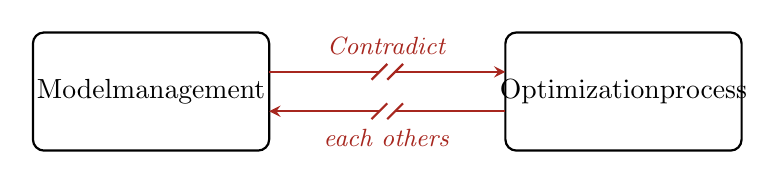
\begin{tikzpicture}
            \draw[thick,rounded corners] (0,0) rectangle (3,1.5);
            \draw[thick,rounded corners] (6,0) rectangle (9,1.5);
            \draw[thick,Mahogany] (3,1) -- (4.4,1);
            \draw[-stealth,thick,Mahogany] (4.6,1) -- (6,1);
            \draw[thick,Mahogany] (4.3,0.9) -- (4.5,1.1);
            \draw[thick,Mahogany] (4.5,0.9) -- (4.7,1.1);
            \draw[thick,Mahogany] (6,0.5) -- (4.6,0.5);
            \draw[-stealth,thick,Mahogany] (4.4,0.5) -- (3,0.5);
            \draw[thick,Mahogany] (4.3,0.4) -- (4.5,0.6);
            \draw[thick,Mahogany] (4.5,0.4) -- (4.7,0.6);
            \node at (1.5,0.75) {\makecell{Model\\ management}};
            \node at (7.5,0.75) {\makecell{Optimization\\ process}};
            \node[above,text=Mahogany] at (4.5,1.1) {\small\emph{Contradict}};
            \node[below,text=Mahogany] at (4.5,0.4) {\small\emph{each others}};
        \end{tikzpicture}
    \end{center}

    \medskip

    These problems are \alert{answered} for COBYQA.
\end{frame}

\begin{frame}
    \frametitle{Our Python implementation}

    We implemented COBYQA in \alert{Python} and made it \alert{publicly available}.
    
	\begin{center}
        \href{https://www.cobyqa.com/}{\includegraphics[width=0.8in]{images/qr/cobyqa.png}}

        \scriptsize\url{https://www.cobyqa.com/}
    \end{center}

    \begin{block}{}
        \textcite{Powell_2006} wrote
        \begin{quote}
            \enquote{The development of NEWUOA has taken nearly \alert{three years}. The work was very \alert{frustrating} [...]}
        \end{quote}
        The development of COBYQA was not easier.
    \end{block}

    It will be included in
    \begin{enumerate}
        \item PDFO as a successor for COBYLA.
        \item GEMSEO, industrial software package for \alert{MDO} (from IRT Saint-Exup{\'{e}}ry).
    \end{enumerate}
\end{frame}

\begin{frame}
    \frametitle{Comparing COBYQA with existing DFO solvers}
    
	\begin{enumerate}
        \item We assess the quality of points based on
        \begin{empheq}[left={\merit(\iter) = \empheqlbrace}]{alignat*=2}
            & \obj(\iter)                           && \quad \text{if~$v_{\infty}(x) \le 10^{-10}$,}\\
            & \infty                                && \quad \text{if~$v_{\infty}(x) \ge 10^{-5}$,}\\
            & \obj(\iter) + 10^5 v_{\infty}(\iter)  && \quad \text{otherwise,}
        \end{empheq}
        where~$v_{\infty}$ denotes the~$\ell_{\infty}$-constraint violation.
        \item The problems are from the \alert{CUTEst} set.
        \item The problems are of \alert{dimension} at most~$50$ (this is \alert{not} small).
        % \item We show the performance profiles for the tolerance~$\tau = 10^{-4}$.
        \item For problems with \alert{inviolable} bounds, we set
        \begin{equation*}
            \obj(\iter) = \infty \quad \text{if~$\xl \nleq \iter$ or~$\iter \nleq \xu$,}
        \end{equation*}
        so that methods that do not respect the bounds do not break down.
    \end{enumerate}
\end{frame}

\begin{frame}
    \frametitle{Performance on bound-constrained problems}

	We make the following comparison on \alert{bound-constrained} problems.

    \medskip

    \begin{center}
        \drawperformanceprofiles{{"COBYQA","BOBYQA","COBYLA","PY-BOBYQA"}}{plain-1-50-perf-bobyqa-cobyla-cobyqa-py-bobyqa-b.csv}{4}
    \end{center}
\end{frame}

\begin{frame}
    \frametitle{Performance on nonlinearly constrained problems}

	We make the following comparison on
    \begin{enumerate}[<+->]
        \item \alert{nonlinearly constrained} problems,
        \item with \alert{inviolable} bounds.
    \end{enumerate}

    \medskip

    \begin{center}
        \only<1>{\drawperformanceprofiles{{"COBYQA","COBYLA"}}{plain-1-50-perf-cobyla-cobyqa-qo.csv}{4}}%
        \only<2>{\drawperformanceprofiles{{"COBYQA","COBYLA"}}{plain-1-50-perf-cobyla-cobyqa-qo-bounds.csv}{4}}
    \end{center}
\end{frame}

\begin{frame}
    \frametitle{Comparison with COBYLA}

	We make the following comparison on \alert{all} problems.

    \medskip

    \begin{center}
        \drawperformanceprofiles{{"COBYQA","COBYLA"}}{plain-1-50-perf-cobyla-cobyqa-ubnlqo.csv}{4}
    \end{center}
\end{frame}

\section{Conclusion and future research directions}

\begin{frame}
    \frametitle{Conclusion}

	We presented the following.
    \begin{enumerate}
        \item \alert{PDFO}, a new interface for using Powell's DFO solvers.
        \begin{enumerate}
            \item It has been downloaded more than \alert{\num{40000} times}.
            \item It is included in the GEMSEO package.
        \end{enumerate}
        \item A theory on the \alert{optimality} of a particular interpolation set.
        \item New perspectives and developments in the \alert{SQP method}.
        \item Our new DFO method \alert{COBYQA}.
        \begin{enumerate}
            \item Numerical experiments show that COBYQA is a \alert{good successor} for COBYLA.
            \item Dr.\ Gallard (MDO architect) from IRT Saint-Exup{\'{e}}ry sent us
        \end{enumerate}
    \end{enumerate}

    \smallskip

    \begin{block}{}
        \begin{quote}
            \small\enquote{I have given it a try and compared with COBYLA on some problems we have (without derivatives), it is significantly faster, provides a better convergence.}
        \end{quote}
    \end{block}
\end{frame}

\begin{frame}
    \frametitle{Future research directions}

    Our thesis opens the door to several interesting future research directions.
    \begin{enumerate}
        \item Study the \alert{convergence} properties of COBYQA.
        \begin{enumerate}
            \item We followed Powell's philosophy when developing COBYQA.
            \item Prove the global convergence of the method.
            \item What is the local convergence rate of COBYQA?
            \item Could we simultaneously have results for COBYLA?
        \end{enumerate}
        \item Look into the \alert{implications} of our new result on the SQP subproblem.
        \begin{enumerate}
            \item How does it connect to \alert{manifold optimization}?
            \item Are these connections related to some convergence theory of COBYQA?
        \end{enumerate}
        \item \dots
        % \item Improve further the \alert{implementation} of COBYQA.
        % \begin{enumerate}
        %     \item The implementation is very complex due to the nature of DFO.
        %     \item How to make it as performant as LINCOA on linearly constrained problems?
        %     \item Implement it in modern Fortran (F2018 or above).
        % \end{enumerate}
    \end{enumerate}
\end{frame}

\appendix

\begin{frame}[t,allowframebreaks]
    \frametitle{References}

	\printbibliography
\end{frame}

\begin{frame}
    \frametitle{Performance on bound-constrained problems}

	We make the following comparison on
    \begin{enumerate}
        \item \alert{bound-constrained} problems,
        \item replacing~$\obj$ with~$[1 + \epsilon(\iter)] \obj(\iter)$ where~$\epsilon(x) \sim N(0, \sigma^2)$,~$\sigma = 10^{-2}$.
    \end{enumerate}

    \medskip

    \begin{center}
        \drawperformanceprofiles{{"COBYQA","BOBYQA","COBYLA"}}{noisy-1-50-2-perf-bobyqa-cobyla-cobyqa-b.csv}{1}
    \end{center}
\end{frame}

\begin{frame}
    \frametitle{Performance on nonlinearly constrained problems}

	We make the following comparison on
    \begin{enumerate}
        \item \alert{nonlinearly constrained} problems,
        \item replacing~$\obj$ with~$[1 + \epsilon(\iter)] \obj(\iter)$ where~$\epsilon(x) \sim N(0, \sigma^2)$,~$\sigma = 10^{-2}$.
    \end{enumerate}

    \medskip

    \begin{center}
        \drawperformanceprofiles{{"COBYQA","COBYLA"}}{noisy-1-50-2-perf-cobyla-cobyqa-qo.csv}{1}
    \end{center}
\end{frame}

\begin{frame}
    \frametitle{Hyperparameter tuning using COBYQA}

    The results on the \enquote{\alert{\only<1>{splice}\only<2>{ijcnn1}}} dataset are summarized below.

    \bigskip

    \begin{center}
        \only<1>{%
            \begin{tabular}{@{}cS[table-format=3]SSS@{}}
                \toprule
                Solver  & {No.\ eval.}  & {AUC score ($10^{-1}$)}   & {Accuracy ($10^{-1}$)}    & {Exec.\ time (\unit{s})}\\
                \midrule
                COBYQA  & 25            & 5.269                     & 5.300                     & 3.037\\
                PDFO    & 65            & 9.568                     & 9.933                     & 3.697\\
                RS      & 100           & 6.409                     & 5.300                     & 4.635\\
                RS      & 300           & 7.880                     & 5.300                     & 13.763\\
                TPE     & 100           & 5.000                     & 5.033                     & 4.889\\
                TPE     & 300           & 7.736                     & 5.300                     & 15.726\\
                \bottomrule
            \end{tabular}%
        }%
        \only<2>{%
            \begin{tabular}{@{}cS[table-format=3]SSS@{}}
                \toprule
                Solver  & {No.\ eval.}  & {AUC score ($10^{-1}$)}   & {Accuracy ($10^{-1}$)}    & {Exec. time (\unit{h})}\\
                \midrule
                COBYQA  & 48            & 9.896                     & 9.779                     & 0.453\\
                PDFO    & 59            & 9.940                     & 9.819                     & 0.526\\
                RS      & 100           & 9.886                     & 9.773                     & 1.231\\
                RS      & 300           & 9.886                     & 9.773                     & 3.681\\
                TPE     & 100           & 9.891                     & 9.791                     & 1.230\\
                TPE     & 300           & 9.896                     & 9.786                     & 3.487\\
                \bottomrule
            \end{tabular}
        }
    \end{center}
\end{frame}

\end{document}